\documentclass[english]{wiasposter}
    % languages: "english" (default), "german", "ngerman"
    % papersize: "a0paper" (default), but you can use other
    % known specifications like "a1paper" or
    % "paperwidth=XXcm,paperheight=YYcm" as optional class argument
\usepackage[utf8]{inputenc}
    % input encoding, maybe you want "latin1" or "ansinew"


\author{Max Mustermann, Moritz Mustermann, Maria Musterfrau}
\title{Big Great Conference}
\logoright{\wgllogo[width=\linewidth]}
\name{Max Mustermann}
\institution{WIAS}
\address{Mohrenstr. 39, 10117 Berlin}
\telephone{+49 30 20372 0}
\email{max.mustermann@wias-berlin.de}
\url{www.wias-berlin.de}

\begin{document}
\wiasframebox{1}{100}{white}{%
}
\wiasframebox{1}{100}{white}{%
}
\wiasframebox{1}{100}{white}{%
}
\wiasframebox{1}{100}{white}{%
}
\wiasframebox{1}{100}{white}{%
}
\wiasframebox{1}{100}{white}{%
}
\wiasframebox{1}{100}{white}{%
}
\wiasframebox{1}{100}{white}{%
}

\wiasframebox{2}{200}{white}{%
Hello, here is some text without a meaning. This text should show, how a
printed text will look like at this place. If you read this text, you will
get no information. Really? Is there no information? Is there a difference
between this text and some nonsense like »Huardest gefburn«? Kjift – Never
mind! A blind text like this gives you information about the selected font,
how the letters are written and the impression of the look. This text
should contain all letters of the alphabet and it should be written in of
the original language. There is no need for a special contents, but the
length of words should match to the language.
}
\wiasbarbox{4}{200}{wiasblue50}{Head}{%
Hello, here is some text without a meaning. This text should show, how a
printed text will look like at this place. If you read this text, you will
get no information. Really? Is there no information? Is there a difference
between this text and some nonsense like »Huardest gefburn«? Kjift – Never
mind! A blind text like this gives you information about the selected font,
how the letters are written and the impression of the look. This text
should contain all letters of the alphabet and it should be written in of
the original language. There is no need for a special contents, but the
length of words should match to the language.
}
\wiasframebox{2}{200}{white}{%
  \begin{itemize}
    \item First item in a list
    \item Second item in a list
    \item Third item in a list
    \item Fourth item in a list
    \item Fivth item in a list
  \end{itemize}
}

\wiascombibox{4}{%
  \wiasframebox{2}{200}{white}{%
    \begin{itemize}
      \item First item in a list
      \item Second item in a list
      \item Third item in a list
      \item Fourth item in a list
      \item Fivth item in a list
    \end{itemize}
  }%
  \wiasframebox{2}{200}{white}{%
    \begin{enumerate}
      \item First item in a list
      \item Second item in a list
      \item Third item in a list
      \item Fourth item in a list
      \item Fivth item in a list
    \end{enumerate}
  }%

  \wiasbarbox{4}{200}{white}{Head}{%
  Hello, here is some text without a meaning. This text should show, how a
  printed text will look like at this place. If you read this text, you will
  get no information. Really? Is there no information? Is there a difference
  between this text and some nonsense like »Huardest gefburn«? Kjift – Never
  mind! A blind text like this gives you information about the selected font,
  how the letters are written and the impression of the look. This text
  should contain all letters of the alphabet and it should be written in of
  the original language. There is no need for a special contents, but the
  length of words should match to the language.
  }%
}
\wiasbarbox{4}{410}{white}{Picture Inclusion}{%
  You can use the normal \LaTeX\ commands for graphics inclusions like
  \texttt{\textbackslash includegraphics}:

  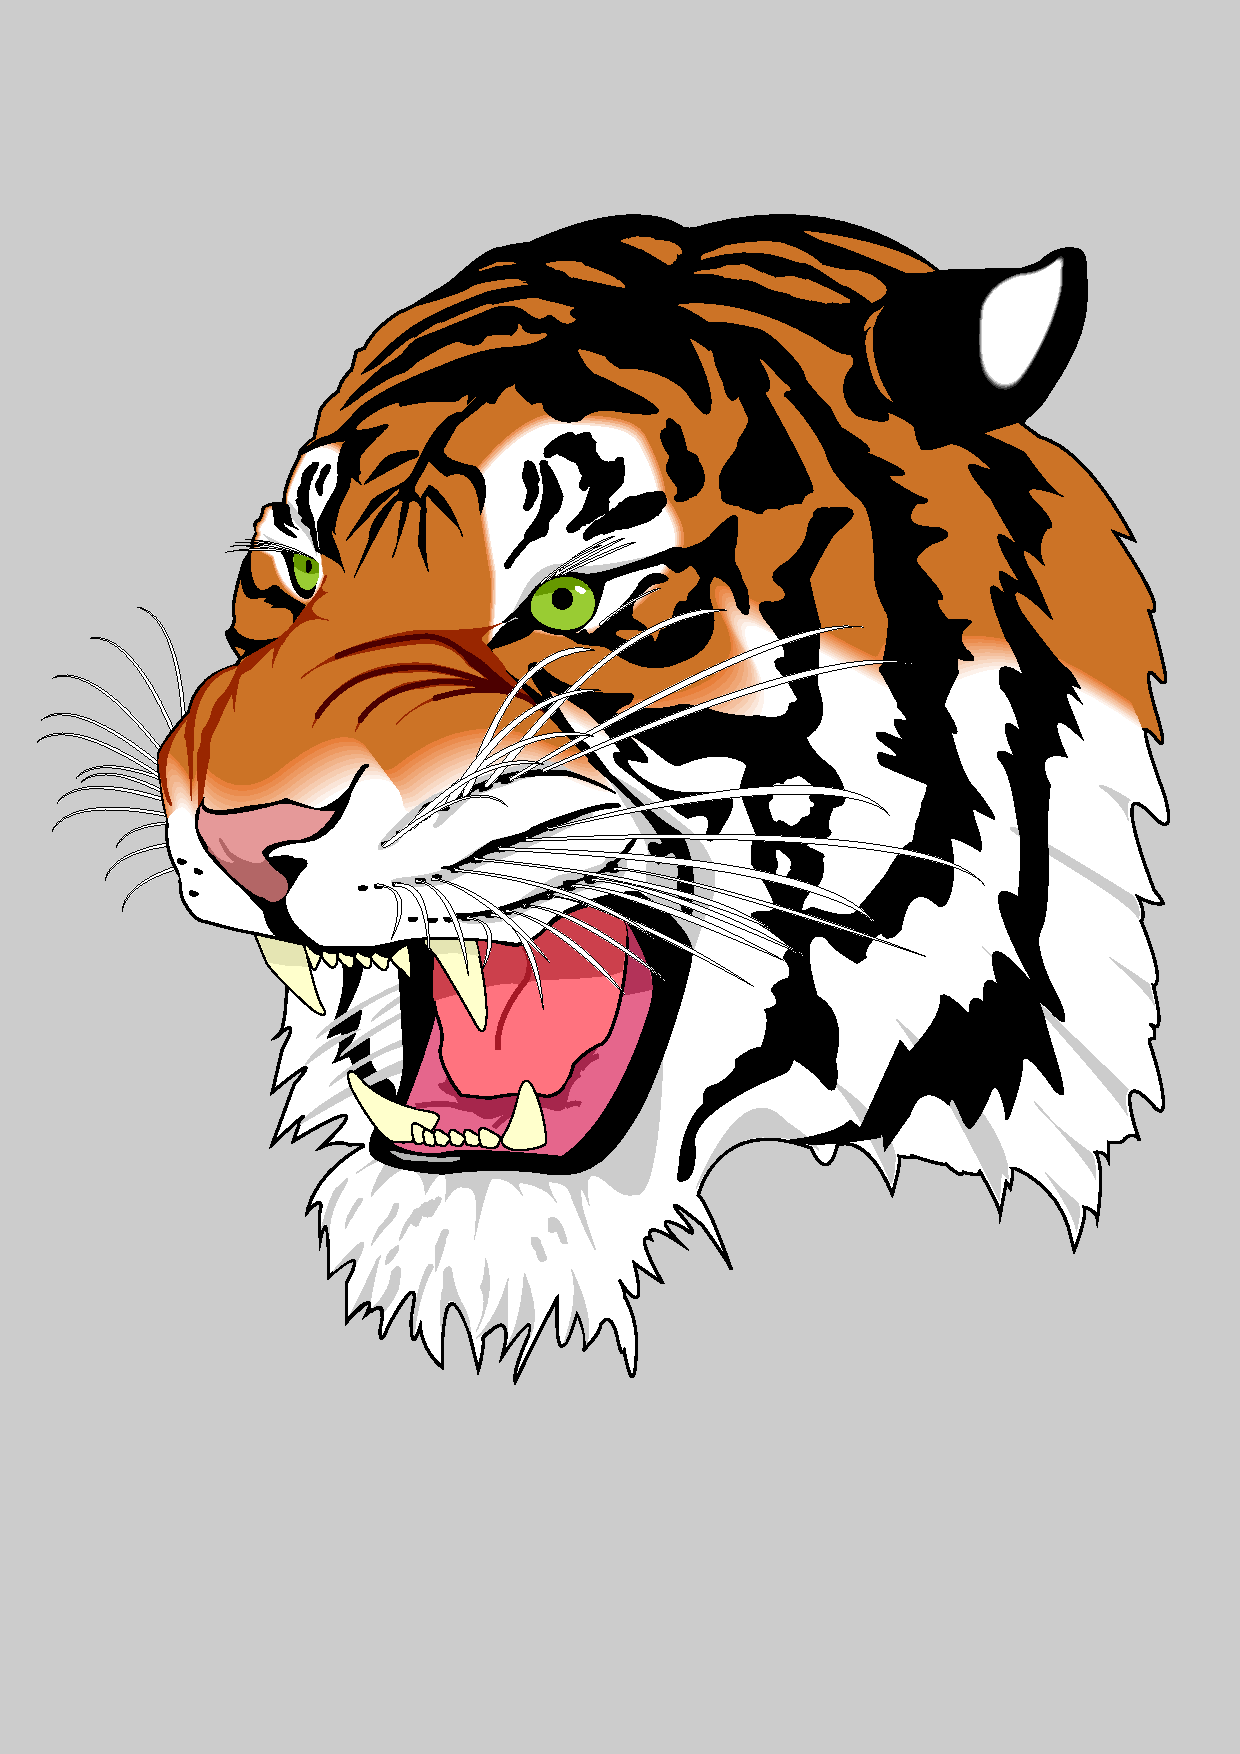
\includegraphics[width=.5\linewidth]{tiger}

  Also you can use the command \texttt{\textbackslash wiaspic}
  (based on wrapfigure) to let text float around the picture.

  \wiaspic{l}{75mm}{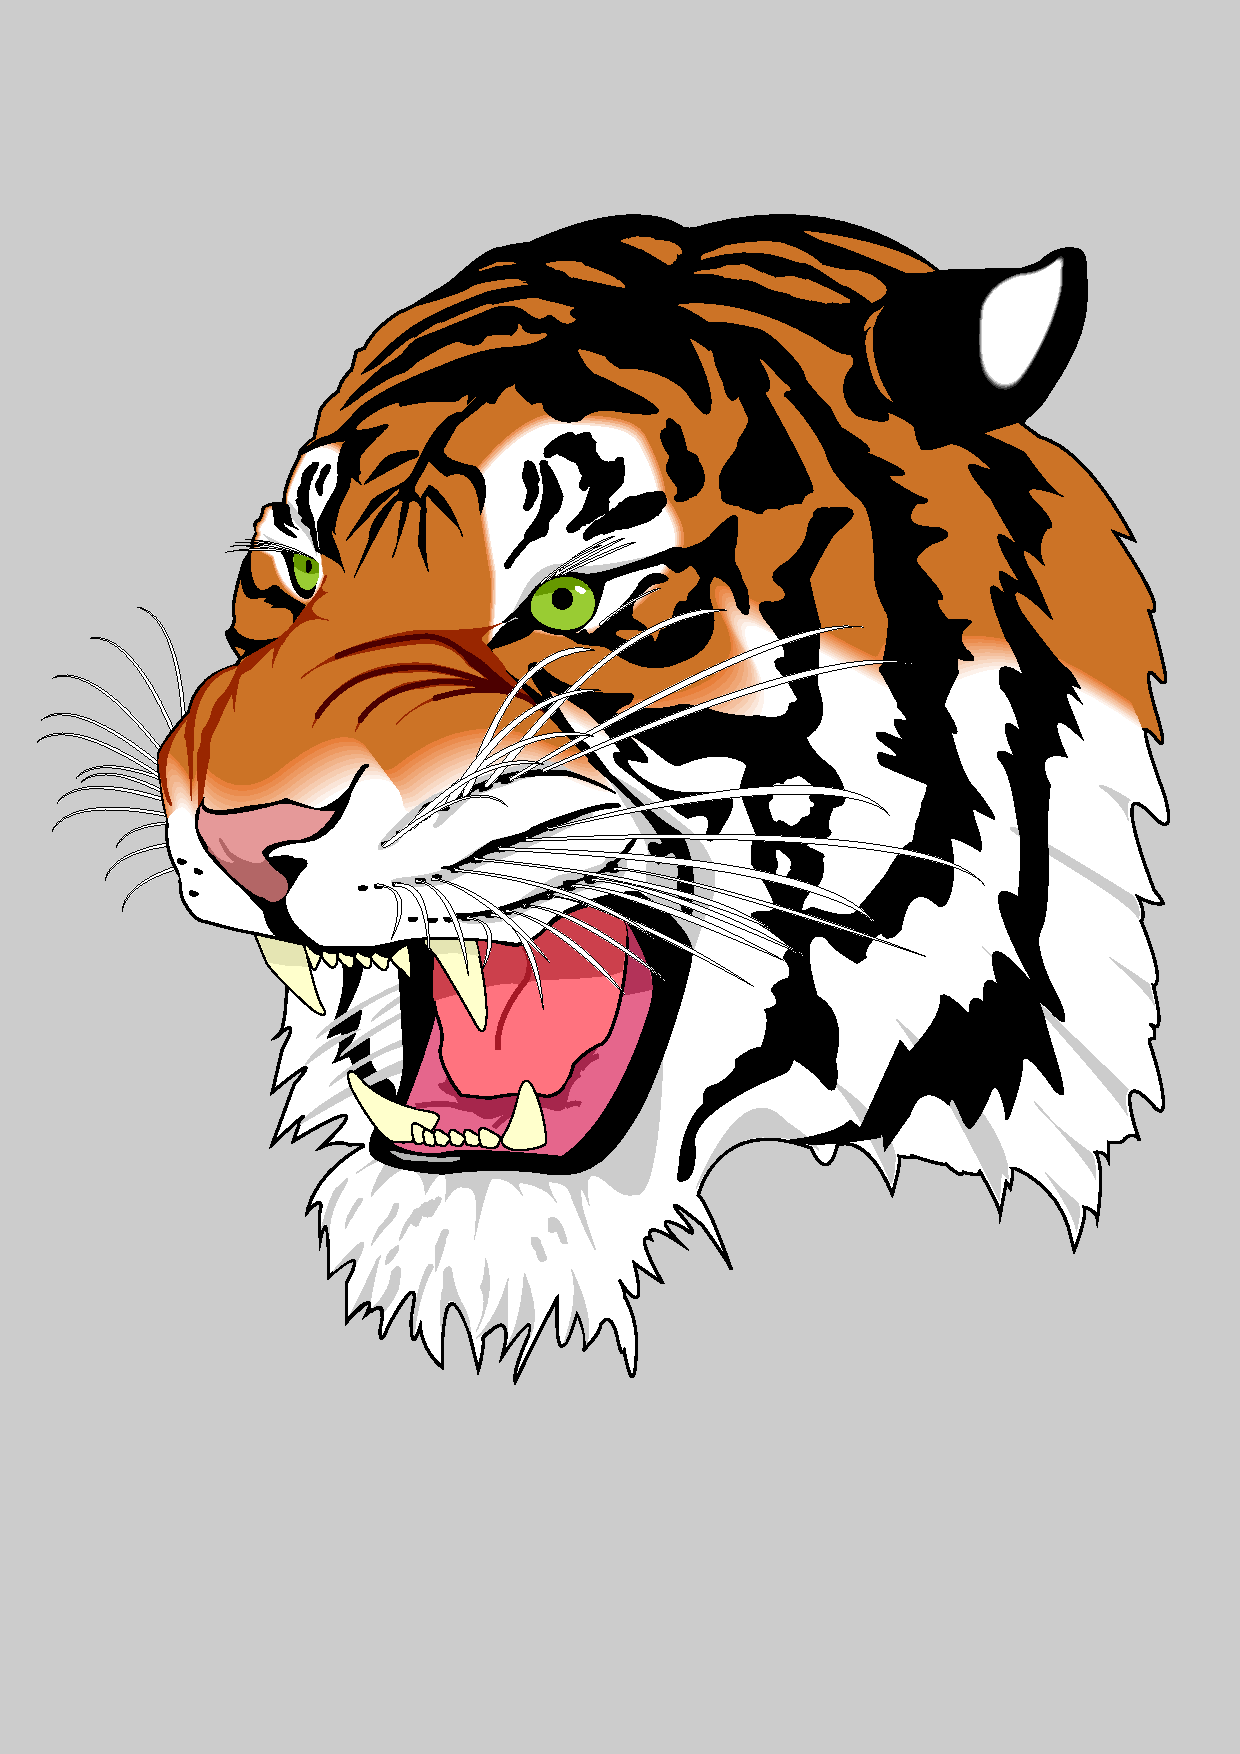
\includegraphics[width=\linewidth]{tiger}}%
  Hello, here is some text without a meaning. This text should show, how a
  printed text will look like at this place. If you read this text, you will
  get no information. Really? Is there no information? Is there a difference
  between this text and some nonsense like »Huardest gefburn«? Kjift – Never
  mind! A blind text like this gives you information about the selected font,
  how the letters are written and the impression of the look. This text
  should contain all letters of the alphabet and it should be written in of
  the original language. There is no need for a special contents, but the
  length of words should match to the language.

  }
\end{document}
